\title{Das kleine Segel 1x1}
%\author{
%}
\date{\today}

\documentclass[12pt]{article}
\usepackage[utf8]{inputenc}
\usepackage[ngerman]{babel}

\usepackage{stmaryrd}
\usepackage{graphicx}
\usepackage{hyperref}
\usepackage{fancybox}
\usepackage{color}
\usepackage{float}

\definecolor{grey}{gray}{0.50}
\setlength{\fboxrule}{2pt}
\newcommand{\xbox}[1]{\vspace{1em}\fcolorbox{grey}{white}{\parbox{0.8\textwidth}{\textcolor{grey}{#1}}}}

\begin{document}
\maketitle

\begin{abstract}
Dieser Text soll eine kurze Einführung in das Thema Segeln sein. Er versucht neuen Seglern die Grundbegriffe näher zu bringen, um mit einen erfahrenen Skipper eine längere Tour durchführen zu können. Am Anfang der Tour werden wir zusätzlich eine praktische Einführung auf dem Boot geben.
\end{abstract}

\xbox{Graue Boxen enthalten zusätzliche Informationen}

%--------------------------------
% GEGENSTÄNDE
%--------------------------------

\section{Gegenstände an Bord}

\paragraph{Tampen}
Seil

\paragraph{Schäkel}
Hiermit werden zum Beispiel Segel mit den Schoten verbunden.
\begin{figure}[H]
\begin{center}
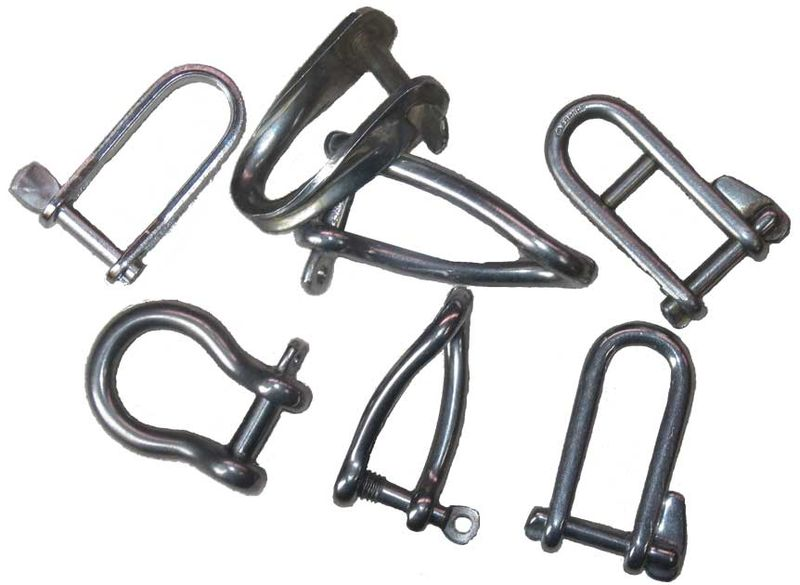
\includegraphics[scale=0.2]{bilder/schaekel.jpg}
\end{center}
\caption{Schäkel}
\label{segel}
\end{figure}

\paragraph{Klampe}
Diese befinden sich häufig an Stegen und auf dem Deck eines Bootes. Sie werden zum festmachen genutzt. Außerdem werden damit die Fallen am Mast fixiert.
Befestigt man einen Tampen an der Klampe spricht man vom Belegen der Klampe.
\begin{figure}[H]
\begin{center}
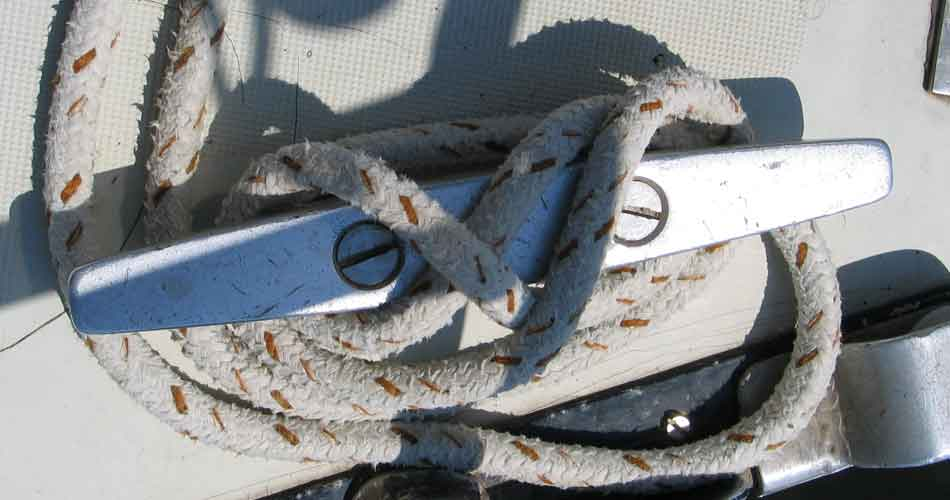
\includegraphics[scale=0.2]{bilder/klampe.jpg}
\end{center}
\caption{Klampe}
\label{segel}
\end{figure}

\paragraph{Fender}

Ein Fender dient als ,,Polsterung" des Bootes zum Steg oder zur Nachbarbooten im Hafen.

\begin{figure}[H]
\begin{center}
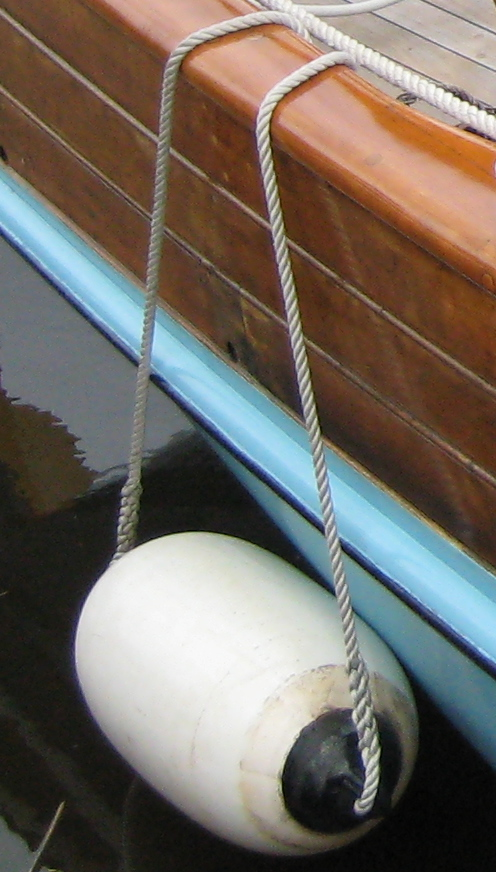
\includegraphics[scale=0.2]{bilder/fender.jpg}
\end{center}
\caption{Fender}
\label{fender}
\end{figure}

\paragraph{Hebelklemme}
Klemmen für Tampen an Bord. Sie sind in der Regel im Cockpit angebracht und fixieren die unter Spannung stehenden Tampen.

\paragraph{Winsch}
Seilwinde im Cockpit zum dichtholen der von Tampen. Die Tampen werden mindestens drei Mal um den Wischkörper geschlungen um die Last aufzunehmen und danach in die Führung gelegt.
Mit Hilfe der Kurbel lässt sich der Tampen nun dichtholen.

\begin{figure}[H]
\begin{center}
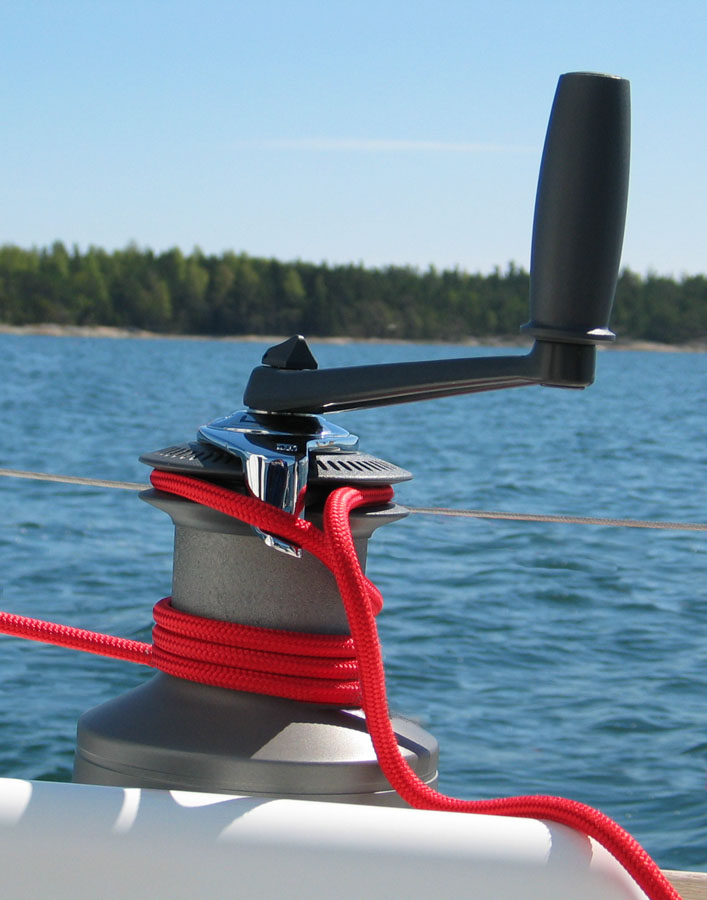
\includegraphics[scale=0.2]{bilder/winch.jpg}
\end{center}
\caption{Winsch}
\label{winsch}
\end{figure}

\xbox{Eine Winsch kann sehr große Kräfte aufnehmen. Deswegen: erst schauen wo es klemmt bevor man mit Gewalt kurbelt.}

%--------------------------------
% BEGRIFFE
%--------------------------------

\section{Wichtige Begriffe}
Dies sind die wichtigsten Begriffe, die alle Mitsegler kennen sollten, damit der Skipper präzise Anweisungen geben kann.

Diese Begriffe und weiteres notwendiges Wissen werden wir auf dem Boot selber erneut besprechen. Dabei werden wir euch auch die notwendigen Knoten beibringen.

Diese Liste soll euch ein Grundgerüst an Wissen vermitteln, daher sind viele Punkte nicht in allen Aspekten erläutert.

\paragraph{Achtknoten, Kreuzknoten, Webeleinstek und Palstek}
Die wichtigstes Knoten an Bord. Mit ihnen lassen sich die meisten Aufgaben lösen.
Es gibt viele Websites mit Anleitungen (z.B. \href{http://www.seasailing.de/knoten.html}{http://www.seasailing.de/knoten.html}).

\paragraph{Bug}
Der vordere Teil des Bootes. Dies bezieht sich auf die Fahrtrichtung also der Teil des Bootes der spitz zuläuft.

\paragraph{Heck}
Der hintere Teil des Bootes. Also die Gegenseite vom Bug.

\paragraph{Backbord}
In Fahrtrichtung gesehen die linke Seite des Bootes. Den Seiten den Bootes werden auch Farben zugewiesen, damit man an Hand von Signallampen nachts die Fahrtrichtung erkennen kann. Die zugewiesene Farbe für Backbord ist \textbf{rot}.

\paragraph{Steuerbord}
In Fahrtrichtung gesehen die rechte Seite des Bootes. Die zugewiesene Farbe für Steuerbord ist \textbf{grün}.

\xbox{Vergisst die Crew Backbord und Steuerbord gibt es vom Skipper - ein Rechtshänder - eine Backpfeife. Nun färbt sich die linke Backe rot. }

\begin{figure}[H]
\begin{center}
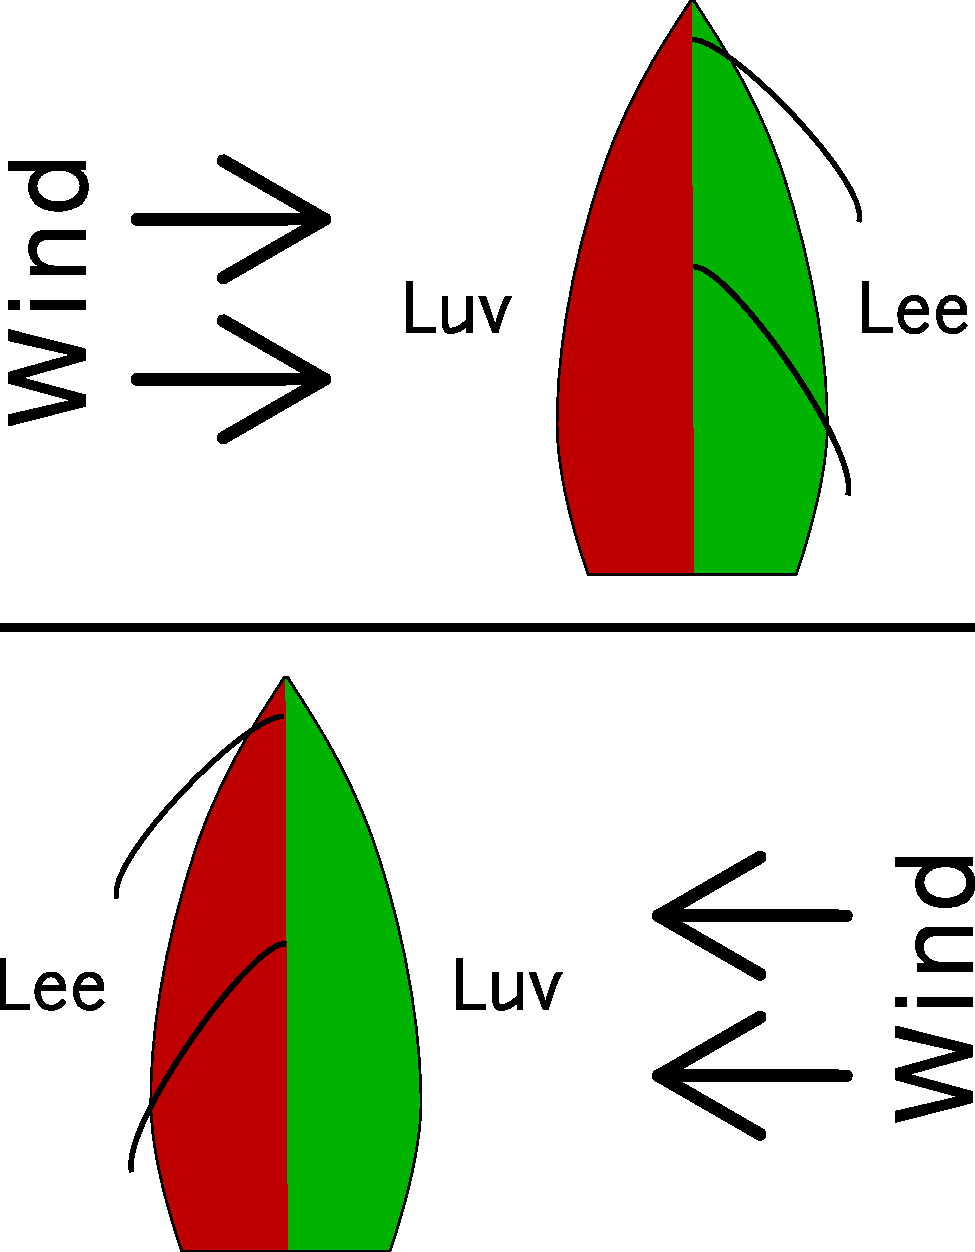
\includegraphics[scale=0.3]{bilder/lee-luv.pdf}
\end{center}
\caption{Lee und Luv / Steuerbord und Backbord}
\label{lee-luv}
\end{figure}

\paragraph{Luv}
Dem Wind zugewandte Seite des Bootes. Kommt der Wind von Backbord, ist dies die Luv-Seite.

\paragraph{Lee}
Dem Wind abgewandte Seite des Bootes.

\begin{quote}
\textbf{Kleine Hilfe:} \textit{Spuckst du in Lee geht's in de See, spuckst du in Luv kommt es wieder ruf.}
\end{quote}

\begin{figure}[H]
\begin{center}
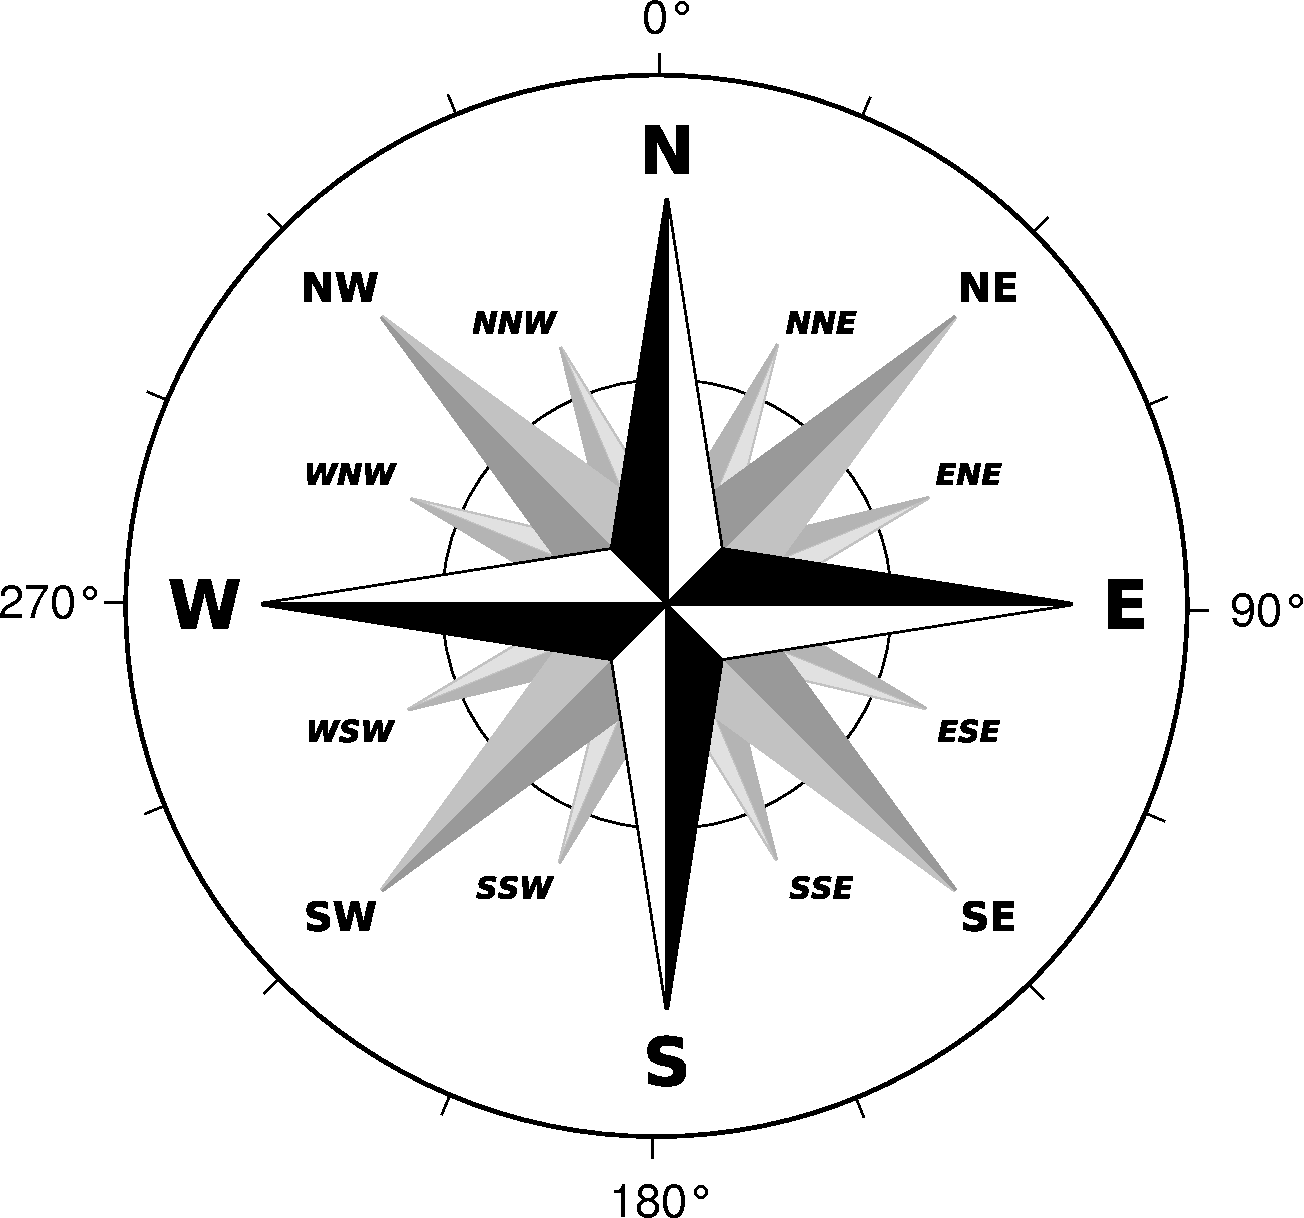
\includegraphics[scale=0.4]{bilder/windrose.pdf}
\caption{Himmelsrichtungen}
\label{himmelsrichtungen}
\end{center}
\end{figure}

\paragraph{Himmelsrichtung}
Hiermit werden Richtungen auf einem Boot angegben. Dies geschieht entweder in Grad(0-360$^\circ$) oder in den gröberen Himmelrichtungen, wie man in Bild \ref{himmelsrichtungen} sieht. Beides bezeichnet den Winkel zum Erdmagnetfeld und kann auf einem Kompass abgelesen werden.

\begin{quote}
\textbf{Achtung:} \textit{Positionen werden auch in Grad(außerdem Minuten und Sekunden) angegeben, hierbei ist allerdings der Winkel auf dem Erdball gemeint.}
\end{quote}

\paragraph{Windrichtung}
Die Windrichtung ist für jeden leicht ersichtlich. Was nicht intuitiv zu verstehen ist, wie die Windrichtung angegeben wird. Die Windrichtung ist die Himmelsrichtung aus der der Wind kommt. Also Windrichtung NE heißt der Wind kommt aus Nord-Ost(North-East).

\paragraph{Kurs}

\begin{figure}[H]
\begin{center}
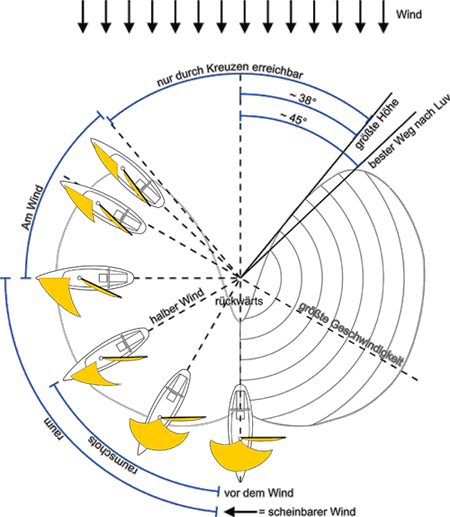
\includegraphics[scale=0.6]{bilder/kurse.png}
\end{center}
\caption{Kurse zur Windrichtung}
\label{kurse}
\end{figure}

Ein Kurs kann auf einen Segelboot zwei Bedeutungen haben. Zum einen bezeichnet es den Kurs den das Schiff zum Magnetfeld der Erde macht. Also die Richtung in Grad, die man auf einem Kompass ablesen kann.

Außerdem kann ein Kurs den Kurs zum Wind bezeichnen. Die Kurse unterscheidet man nach dem Winkel zwischen der Windrichtung und Fahrtrichtung des Bootes. Diese Kurse zum Wind werden nur grob in Am-Wind-Kurs, Halbwindkurs, Raumwindkurs und Vorwindkurs eingeteilt, aber dies werdet ihr auf dem Boot kennen lernen.

\xbox{Abbildung \ref{kurse} zeigt die Kurse zum Wind. Auf der linken Seite sind die Kurse auf Backbordbug (Segel werden auf Backbord - die linke Seite des Bootes - gefahren) gezeigt. Die Kurse auf Steuerbordbug werden nicht gezeigt. Ein Wechsel des Bugs wird Wende genannt, wenn er mit dem Bug durch den Wind geschieht (im Diagramm oben). Dreht sich beim Bugwechsel das Heck durch den Wind spricht man von einer Halse. Siehe auch \texttt{Wende und Halse}}

\paragraph{Schot}
Damit das Boot optimal voran kommt, muss das Segel passend zum Kurs zum Wind eingestellt werden.

Dies geschieht über Schoten - Tampen, die an den Segeln befestigt sind. Jedes Segel hat eigene Schoten. Eine Übersicht über alle Schoten findet ihr in Bild \ref{schoten}.

\begin{figure}[h!]
\begin{center}
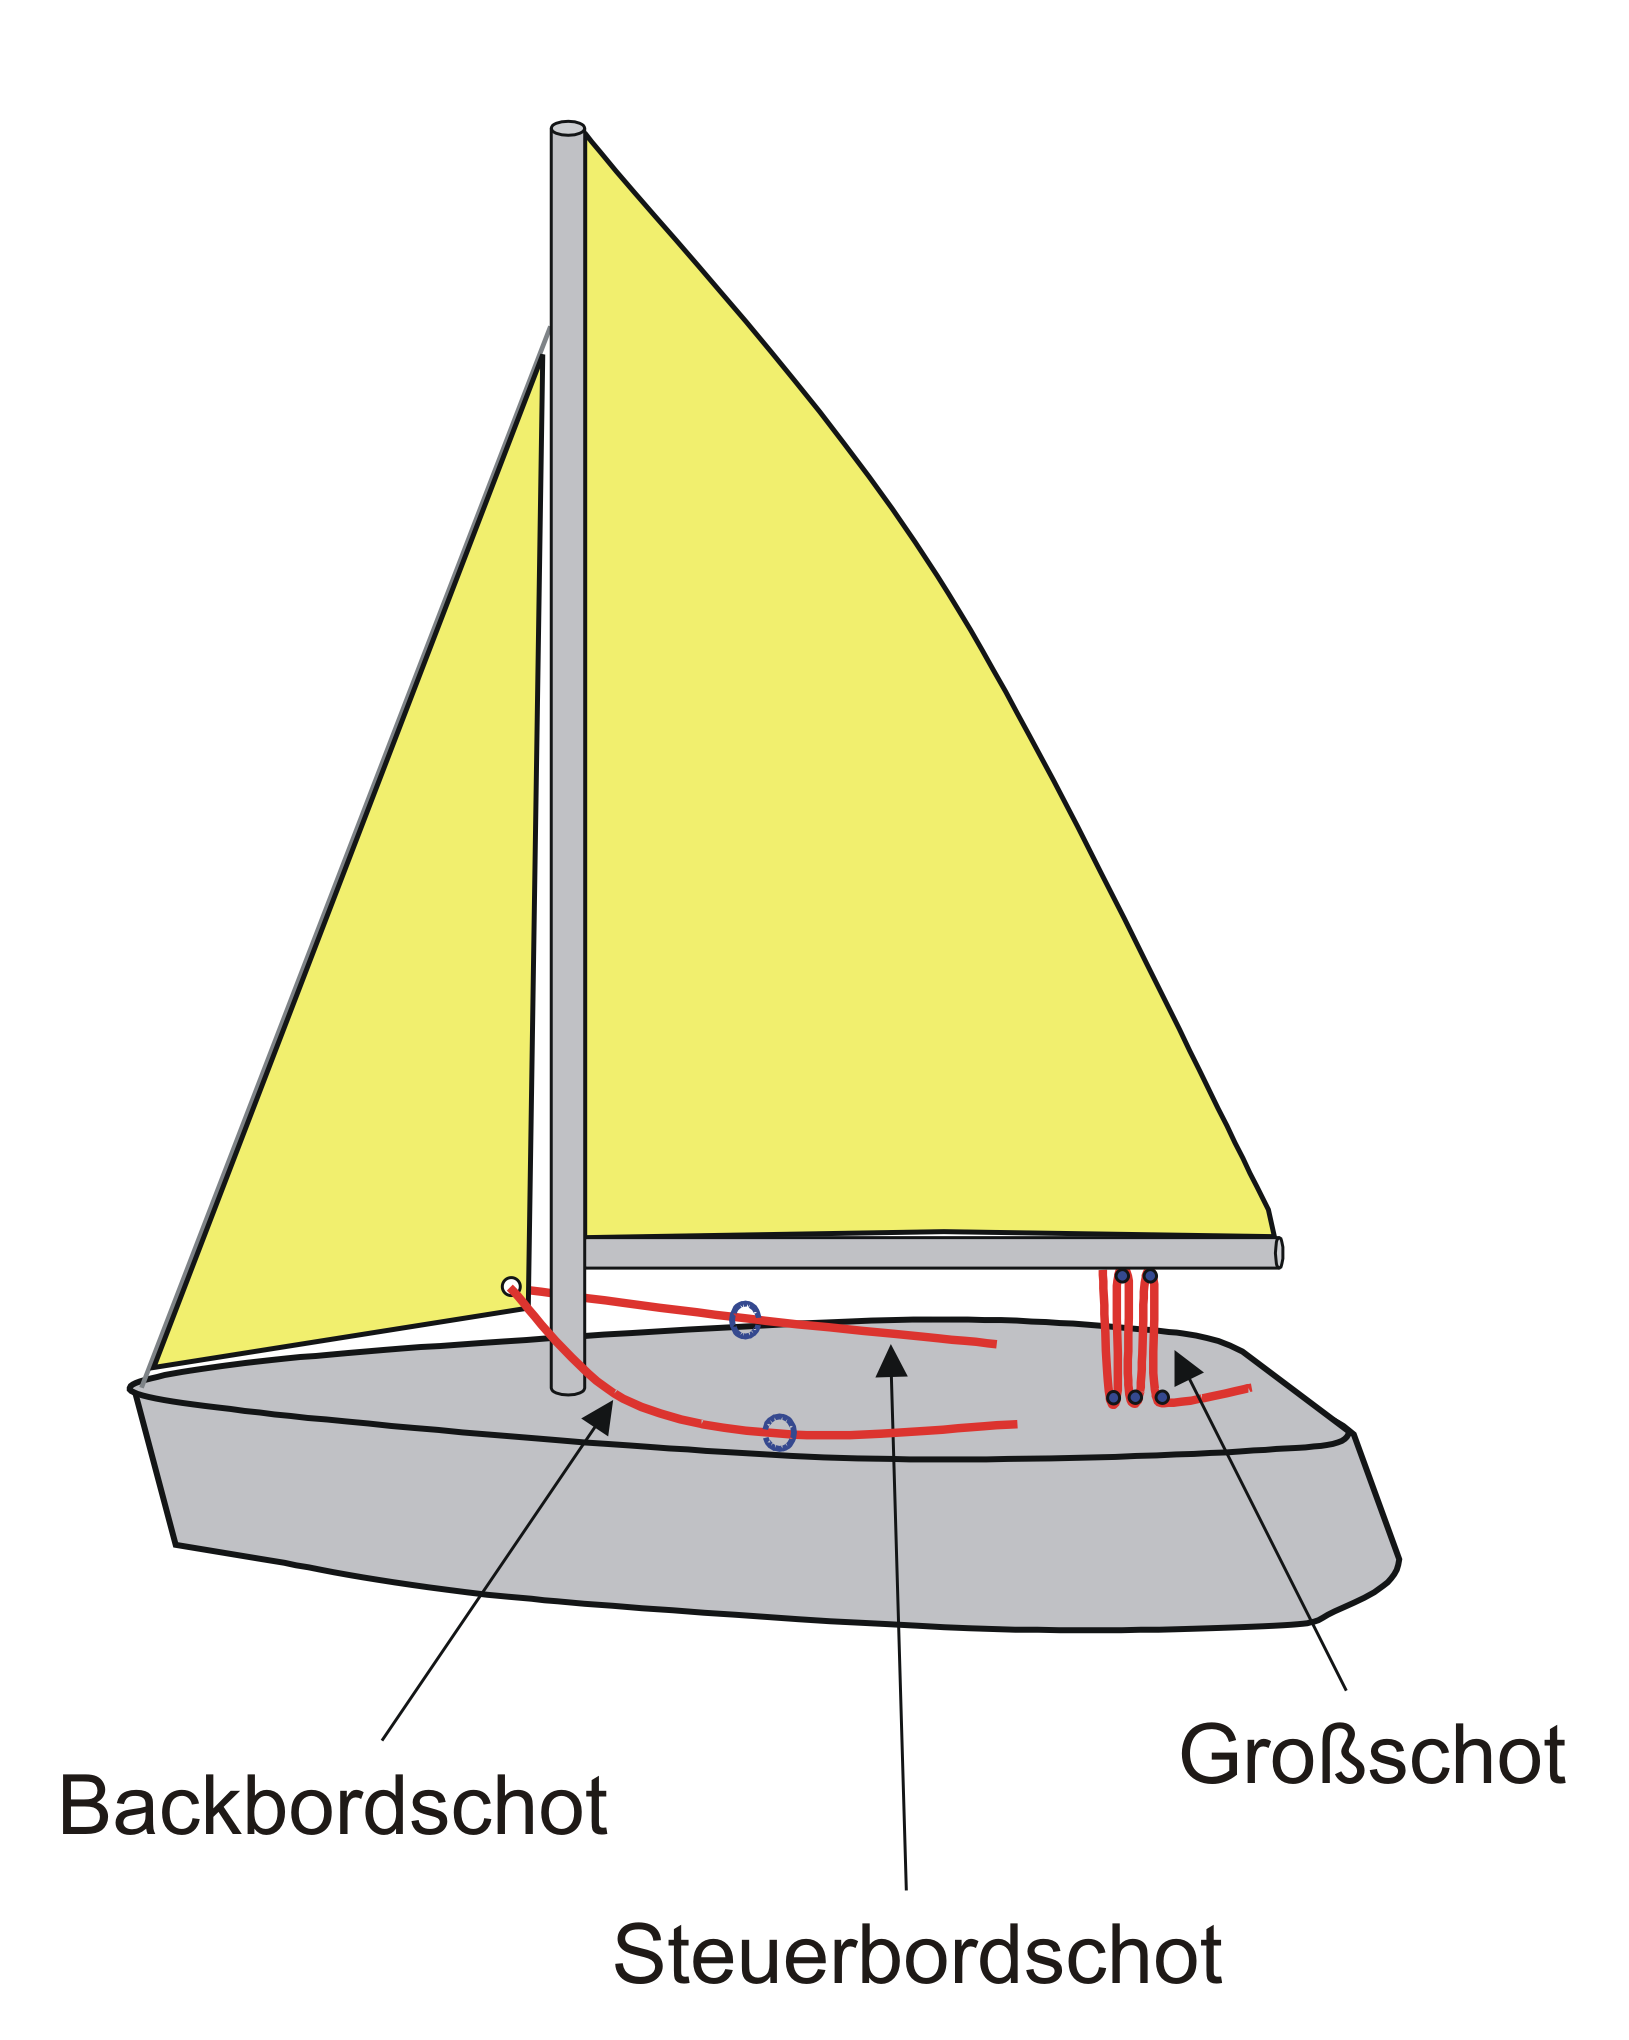
\includegraphics[scale=0.4]{bilder/schoten.png}
\end{center}
\caption{Die Schoten einer Yacht}
\label{schoten}
\end{figure}

\paragraph{Vorleine und Achterleine}
Diese Tampen werden zum Festmachen des Bootes genutzt. Die Vorderleinen werden an der Bugklampe belegt und am Steg befestigt. Die Achterleinen werden auf den Heckklampen belegt und um einen Pfahl gelegt.

\xbox{Je nach Gegebenheiten im Hafen werden andere Leinen ausgelegt. Vor jedem Anlegemanöver werden wir die Reihenfolge und Anzahl der Leinen mit euch besprechen.}

\paragraph{Fallen}
Um die Segel aufzuspannen sind sie oben an der Mastspitze(\textit{Mast} siehe Bild \ref{segel}) befestigt. Diese Befestigungen werden mit Tampen realisiert, die von der Mastspitze am Mast entlang oder im Mast geführt werden. Diese Tampen werden Fallen genannt.

\paragraph{Wanten und Stagen (Stehendes Gut)}
Der Mast wird mit Stahlseilen am Boot verspannt. Würde man dies nicht tun, würde der Mast beim Segeln unter der Belastung abbrechen.

Die Stagen spannen den Mast nach Vorne und Hinten ab, die Wanten zu den Seiten. In Bild \ref{segel} ist das Backbord-Want und das Vorstag, also das vordere Stag, eingezeichnet.

%--------------------------------
% MANÖVER
%--------------------------------

\section{Manöver}

\paragraph{Skipper}
Der Skipper trägt die zivil- und strafrechtliche Verantwortung für die Sicherheit von Schiff und Besatzung.

\paragraph{Wende und Halse}
Dies sind Manöver, bei denen die Segel die Seite des Bootes wechseln. Kommt der Wind erst von Backbord, kommt er danach von Steuerbord. Findet dieser Seitenwechsel nicht statt, ist es keine Halse oder Wende.

\paragraph{Anluven}
Manöver bei dem der Winkel zwischen Fahrtrichtung und Wind \textbf{verkleinert} wird.

\paragraph{Abfallen}
Manöver bei dem der Winkel zwischen Fahrtrichtung und Wind \textbf{vergrößert} wird.

%--------------------------------
% SEGEL
%--------------------------------

\section{Die Segel}

\begin{figure}[h!]
\begin{center}
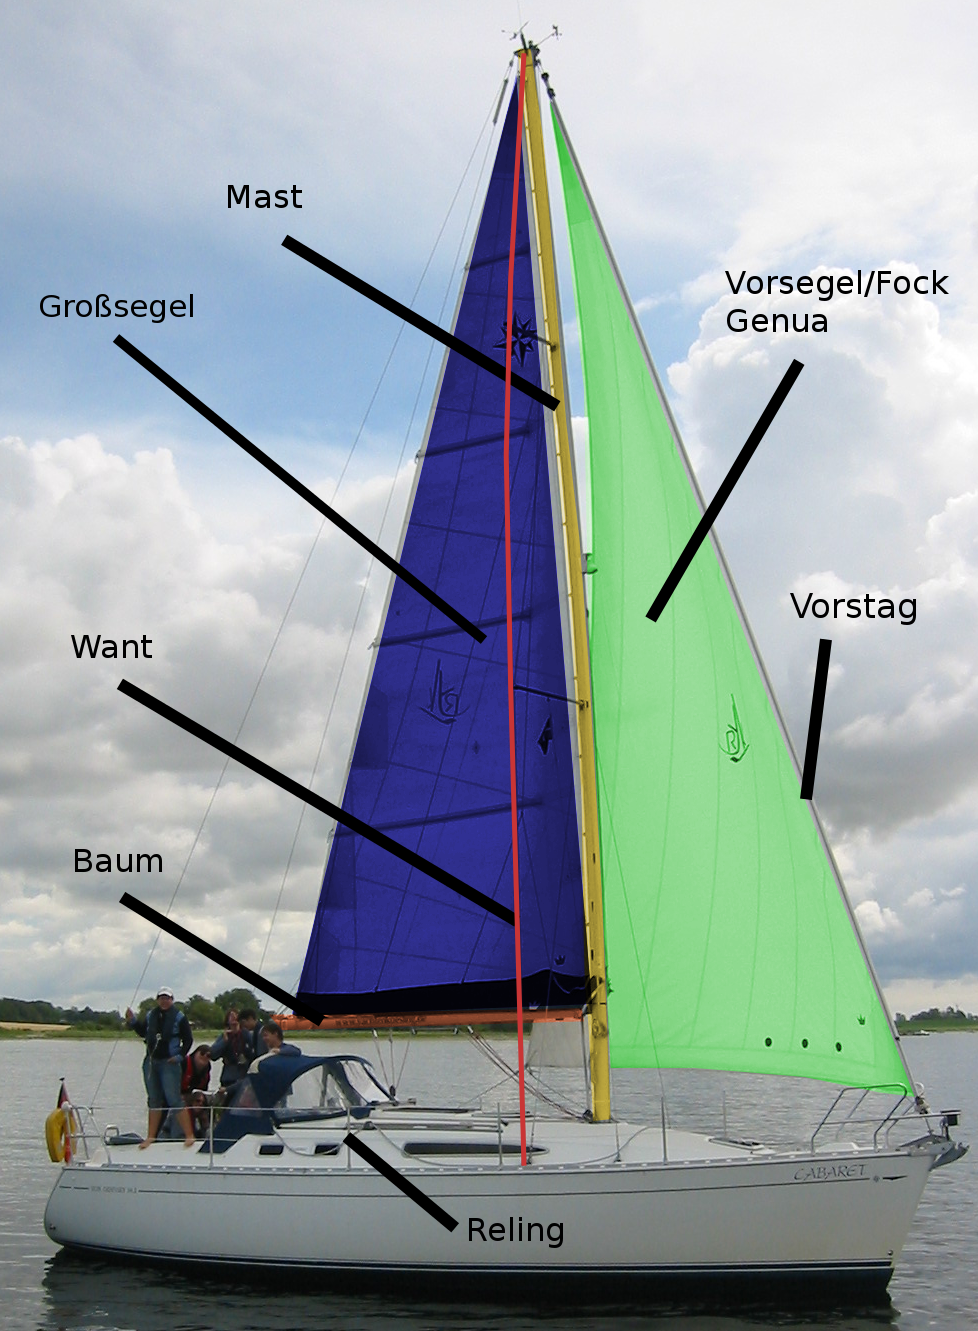
\includegraphics[scale=0.2]{bilder/yacht.png}
\end{center}
\caption{Die Segel einer Yacht}
\label{segel}
\end{figure}

Eine moderne Segelyacht hat zwei Segel. Ein Großsegel und ein Vorsegel.
Das Vorsegel wird je nach Größe auch Fock oder Genua genannt.

Das Großsegel wird hinter dem Mast gefahren. An der Unterkante des Segels befindet sich der Baum.

\section{Verhalten an Bord}
Um Unfälle zu vermeiden gibt es einige Verhaltensregeln: Die wohl
wichtigste Regel lautet:
\begin{quote}
\textit{Eine Hand fürs Boot und eine für sich selber.}
\end{quote}
Dies bedeutet, dass ihr bei allem was ihr an Bord macht (Segel setzen,
beim Anlegen im Hafen einen Knoten machen, usw.), immer auch auf eure
eigene Sicherheit achtet: Auf sicheren Stand achten, Festhalten, sich im Zweifel helfen lassen.
\begin{quote}
\textit{Den Anweisungen eures Skippers Folge leisten.}
\end{quote}
In brenzligen Situationen kommt es auf jede Sekunde an und
manchmal ist der Sinn einer Anweisung nicht ganz ersichtlich. Wenn erst diskutiert werden muss, kann schnell etwas schief gehen. Im Zweifelsfall sollte euer Skipper wissen was er tut. Die Zeit für Diskussionen über Sinn und Unsinn ist abends im Hafen. Dort sollte man dann auch nicht mit Kritik sparen.

\begin{quote}
\textit{Rückmeldungen geben.}
\end{quote}
Es ist in engen Situation wichtig, dass der Skipper/Steuermann/Steuerfrau alles im Blick hat. Gerade bei großen Yachten ist dies teilweise sehr schwierig. Deswegen sollte jeder an Bord versuchen wichtige Beobachtungen (z.B. Kollisionsgefahr) und Statusmeldungen (z.B. Segel gesetzt) unverzüglich, deutlich und laut an den Steuermann/Steuerfrau zu melden.

\section{Packliste}
Dies ist eine Liste der Sachen an die man unbedingt denken muss. Sie ist nur eine Referenz und erhebt keinen Anspruch auf Vollständigkeit. Als Transportmittel nutzt ihr bitte eine \textbf{flexible Tasche/Rucksack/Seesack}. Hartschalenkoffer lassen sich sehr schlecht verstauen.

\subsection*{Was ist schon da?}
\begin{itemize}
\renewcommand{\labelitemi}{$\boxempty$}
\item Schwimmweste
\item Geschirr und Besteck
\item Matratze
\end{itemize}

\subsection*{Was muss?}
Wichtig sind hierbei vor allem die Regensachen (wasserdichte Schuhe, Kopfbedeckung, Jacke und Hose). Falls es regnen sollte, macht die Tour ohne keinen Spaß mehr. Diese sollten möglichst robust sein, damit sie nicht sofort zerreißen.
\begin{itemize}
\renewcommand{\labelitemi}{$\boxempty$}
\item Schlafsack
\item Bettlaken
\item Kissen
\item Brillenband
\item Waschsachen
\item Badesachen
\item Regenjacke(am besten eine feste) mit Kapuze oder Südwester
\item Regenhose
\item Gummistiefel
\item Schuhe mit abriebfester Sohle
\item Genug warme Sachen (eine Mütze ist vielleicht auch angebracht)
\end{itemize}

\subsection*{Was kann?}
\begin{itemize}
\renewcommand{\labelitemi}{$\boxempty$}
\item Segelhandschuhe

\end{itemize}

Eine zusätzliche Inspiration kann diese Liste sein: \href{http://www.pc-ostsee.de/yachtcharter/sites/download/Packliste.pdf}{Packliste PCO}

\end{document}
